\documentclass[11pt,a4paper]{article}

% Page geometry
\usepackage[margin=0.75in]{geometry}

% Fonts
\usepackage{fontspec}
\setmainfont{Helvetica Neue}[
    BoldFont = Helvetica Neue Bold,
    ItalicFont = Helvetica Neue Italic
]

% Colors - JASPER brand
\usepackage{xcolor}
\definecolor{jaspernavy}{HTML}{0F172A}
\definecolor{jasperemeralddark}{HTML}{1E6B45}
\definecolor{jasperemerald}{HTML}{2C8A5B}
\definecolor{jasperslate}{HTML}{64748B}
\definecolor{jaspergray}{HTML}{F8FAFC}
\definecolor{jaspergold}{HTML}{F59E0B}

% Category colors
\definecolor{catgov}{HTML}{F59E0B}
\definecolor{catbuild}{HTML}{3B82F6}
\definecolor{catfund}{HTML}{8B5CF6}
\definecolor{catops}{HTML}{EF4444}
\definecolor{catwc}{HTML}{A855F7}
\definecolor{catfs}{HTML}{1E1E1E}
\definecolor{catanalysis}{HTML}{F97316}
\definecolor{catoutput}{HTML}{06B6D4}

% Graphics
\usepackage{graphicx}
\usepackage{tikz}
\usetikzlibrary{shapes.geometric, arrows.meta, positioning, fit, backgrounds}

% Tables
\usepackage{tabularx}
\usepackage{booktabs}
\usepackage{array}
\usepackage{colortbl}
\usepackage{multirow}
\usepackage{longtable}

% Lists
\usepackage{enumitem}
\setlist[itemize]{leftmargin=*, itemsep=1pt, topsep=2pt}

% Hyperlinks
\usepackage{hyperref}
\hypersetup{
    colorlinks=true,
    linkcolor=jasperemerald,
    urlcolor=jasperemerald
}

% Header/Footer
\usepackage{fancyhdr}
\pagestyle{fancy}
\fancyhf{}
\renewcommand{\headrulewidth}{0pt}
\fancyfoot[C]{\textcolor{jasperslate}{\small JASPER Financial Architecture | The 28-Sheet Model Guide}}
\fancyfoot[R]{\textcolor{jasperslate}{\small Page \thepage}}

\begin{document}

% Title Page
\begin{center}
    \includegraphics[width=3cm]{../images/jasper-logo.png}\\[8pt]

    {\fontsize{32}{38}\selectfont\textcolor{jaspernavy}{\textbf{JASPER}}}\\[4pt]
    {\small\textcolor{jasperslate}{FINANCIAL ARCHITECTURE}}\\[32pt]

    \colorbox{jaspernavy}{%
        \parbox{0.85\linewidth}{%
            \centering\vspace{8pt}
            \textcolor{white}{\fontsize{20}{24}\selectfont\bfseries The 28-Sheet Financial Model}\\[4pt]
            \textcolor{jasperemerald}{\large Architecture Guide}
            \vspace{8pt}
        }%
    }\\[16pt]

    {\large\textcolor{jasperslate}{\itshape DFI-Grade Infrastructure Financial Modelling}}
\end{center}

\vspace{24pt}

% Introduction Box
\noindent\colorbox{jaspergray}{%
    \parbox{\dimexpr\linewidth-2\fboxsep}{%
        \vspace{8pt}
        \textcolor{jaspernavy}{\bfseries What is the JASPER 28-Sheet Architecture?}\\[6pt]
        \textcolor{jaspernavy}{The JASPER 28-Sheet Architecture is a comprehensive, standardised financial model structure designed to meet Development Finance Institution (DFI) requirements. It organises all project financials into eight logical categories, ensuring complete audit trails, balanced financial statements, and professional presentation.}
        \vspace{8pt}
    }%
}

\vspace{20pt}

% Architecture Overview
\section*{\textcolor{jaspernavy}{Model Architecture Overview}}

\begin{center}
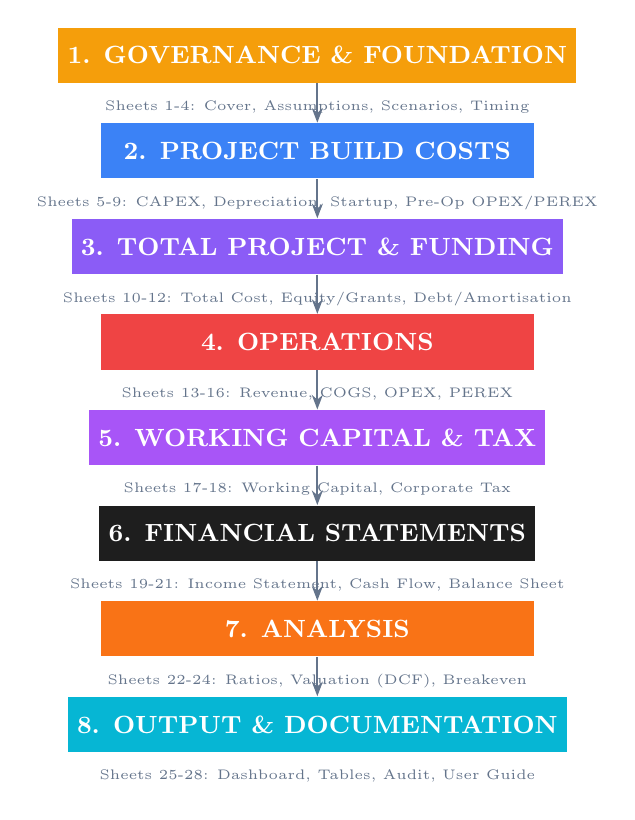
\begin{tikzpicture}[
    node distance=0.3cm,
    box/.style={rectangle, draw=none, minimum width=5.5cm, minimum height=0.7cm, text=white, font=\small\bfseries, align=center},
    arrow/.style={-{Stealth[scale=0.8]}, thick, draw=jasperslate}
]

% Category 1: Governance
\node[box, fill=catgov] (gov) {1. GOVERNANCE \& FOUNDATION};
\node[below=0.1cm of gov, font=\tiny\color{jasperslate}] {Sheets 1-4: Cover, Assumptions, Scenarios, Timing};

% Category 2: Build
\node[box, fill=catbuild, below=0.5cm of gov] (build) {2. PROJECT BUILD COSTS};
\node[below=0.1cm of build, font=\tiny\color{jasperslate}] {Sheets 5-9: CAPEX, Depreciation, Startup, Pre-Op OPEX/PEREX};

% Category 3: Funding
\node[box, fill=catfund, below=0.5cm of build] (fund) {3. TOTAL PROJECT \& FUNDING};
\node[below=0.1cm of fund, font=\tiny\color{jasperslate}] {Sheets 10-12: Total Cost, Equity/Grants, Debt/Amortisation};

% Category 4: Operations
\node[box, fill=catops, below=0.5cm of fund] (ops) {4. OPERATIONS};
\node[below=0.1cm of ops, font=\tiny\color{jasperslate}] {Sheets 13-16: Revenue, COGS, OPEX, PEREX};

% Category 5: WC & Tax
\node[box, fill=catwc, below=0.5cm of ops] (wc) {5. WORKING CAPITAL \& TAX};
\node[below=0.1cm of wc, font=\tiny\color{jasperslate}] {Sheets 17-18: Working Capital, Corporate Tax};

% Category 6: Financials
\node[box, fill=catfs, below=0.5cm of wc] (fs) {6. FINANCIAL STATEMENTS};
\node[below=0.1cm of fs, font=\tiny\color{jasperslate}] {Sheets 19-21: Income Statement, Cash Flow, Balance Sheet};

% Category 7: Analysis
\node[box, fill=catanalysis, below=0.5cm of fs] (analysis) {7. ANALYSIS};
\node[below=0.1cm of analysis, font=\tiny\color{jasperslate}] {Sheets 22-24: Ratios, Valuation (DCF), Breakeven};

% Category 8: Output
\node[box, fill=catoutput, below=0.5cm of analysis] (output) {8. OUTPUT \& DOCUMENTATION};
\node[below=0.1cm of output, font=\tiny\color{jasperslate}] {Sheets 25-28: Dashboard, Tables, Audit, User Guide};

% Arrows
\draw[arrow] (gov.south) -- (build.north);
\draw[arrow] (build.south) -- (fund.north);
\draw[arrow] (fund.south) -- (ops.north);
\draw[arrow] (ops.south) -- (wc.north);
\draw[arrow] (wc.south) -- (fs.north);
\draw[arrow] (fs.south) -- (analysis.north);
\draw[arrow] (analysis.south) -- (output.north);

\end{tikzpicture}
\end{center}

\newpage

% Detailed Sheet Breakdown
\section*{\textcolor{jaspernavy}{Complete 28-Sheet Breakdown}}

% Category 1
\subsection*{\colorbox{catgov}{\textcolor{white}{\small\bfseries 1. GOVERNANCE \& FOUNDATION}} \textcolor{catgov}{\small (Sheets 1-4)}}

\begin{tabularx}{\linewidth}{@{}p{2.5cm}X@{}}
\textbf{Sheet 1} & \textbf{Cover \& Index} - Project identity, version control, hyperlinked index to all sheets \\[4pt]
\textbf{Sheet 2} & \textbf{Assumptions} - All model inputs in one location. Guiding note: Each sheet may only reference sheets above. Sources documented. \\[4pt]
\textbf{Sheet 3} & \textbf{Scenarios \& Sensitivities} - Base/Upside/Downside cases, data tables for sensitivity analysis \\[4pt]
\textbf{Sheet 4} & \textbf{Timing \& Flags} - Project phases, period flags, construction vs operations timeline \\
\end{tabularx}

\vspace{12pt}

% Category 2
\subsection*{\colorbox{catbuild}{\textcolor{white}{\small\bfseries 2. PROJECT BUILD COSTS}} \textcolor{catbuild}{\small (Sheets 5-9)}}

\begin{tabularx}{\linewidth}{@{}p{2.5cm}X@{}}
\textbf{Sheet 5} & \textbf{CAPEX} - Capital expenditures. Formula: Quantity $\times$ Unit Cost $\times$ (1+Escalation)\^{}Year + Contingency \\[4pt]
\textbf{Sheet 6} & \textbf{Depreciation} - Asset depreciation schedules. Formula: CAPEX $\times$ AssetCost / UsefulLife \\[4pt]
\textbf{Sheet 7} & \textbf{Startup Costs} - One-time initial costs before operations (marketing, training, licences) \\[4pt]
\textbf{Sheet 8} & \textbf{Pre-Op OPEX} - Operating expenses incurred before revenue generation (staff, utilities, rent) \\[4pt]
\textbf{Sheet 9} & \textbf{Pre-Op PEREX} - Personnel expenses incurred before revenue generation \\
\end{tabularx}

\vspace{12pt}

% Category 3
\subsection*{\colorbox{catfund}{\textcolor{white}{\small\bfseries 3. TOTAL PROJECT \& FUNDING}} \textcolor{catfund}{\small (Sheets 10-12)}}

\begin{tabularx}{\linewidth}{@{}p{2.5cm}X@{}}
\textbf{Sheet 10} & \textbf{Total Project Cost} - Aggregation of all build costs. Formula: CAPEX + Startup + IDC + Pre-Op OPEX + Pre-Op PEREX \\[4pt]
\textbf{Sheet 11} & \textbf{Equity \& Grants} - Equity injections and grant funding schedules \\[4pt]
\textbf{Sheet 12} & \textbf{Debt \& Amortisation} - Loan schedules, interest, principal repayments. Contains circular reference with Cash (solved by Python engine). \\
\end{tabularx}

\vspace{12pt}

% Category 4
\subsection*{\colorbox{catops}{\textcolor{white}{\small\bfseries 4. OPERATIONS}} \textcolor{catops}{\small (Sheets 13-16)}}

\begin{tabularx}{\linewidth}{@{}p{2.5cm}X@{}}
\textbf{Sheet 13} & \textbf{Revenue} - All revenue streams. Formula: Volume $\times$ Price $\times$ (1+Escalation)\^{}Year \\[4pt]
\textbf{Sheet 14} & \textbf{COGS} - Cost of goods sold. Typically \% of Revenue or unit-based \\[4pt]
\textbf{Sheet 15} & \textbf{OPEX} - Operating expenses post-operations. Target \% of Revenue benchmarks \\[4pt]
\textbf{Sheet 16} & \textbf{PEREX} - Personnel expenses post-operations. Headcount $\times$ Salary with escalation \\
\end{tabularx}

\vspace{12pt}

% Category 5
\subsection*{\colorbox{catwc}{\textcolor{white}{\small\bfseries 5. WORKING CAPITAL \& TAX}} \textcolor{catwc}{\small (Sheets 17-18)}}

\begin{tabularx}{\linewidth}{@{}p{2.5cm}X@{}}
\textbf{Sheet 17} & \textbf{Working Capital} - Receivables, Inventory, Payables. Formula: WC = Receivables + Inventory - Payables \\[4pt]
\textbf{Sheet 18} & \textbf{Tax} - Corporate tax calculations, tax losses carried forward \\
\end{tabularx}

\newpage

% Category 6
\subsection*{\colorbox{catfs}{\textcolor{white}{\small\bfseries 6. FINANCIAL STATEMENTS}} \textcolor{catfs}{\small (Sheets 19-21)}}

\begin{tabularx}{\linewidth}{@{}p{2.5cm}X@{}}
\textbf{Sheet 19} & \textbf{Income Statement (IS)} - P\&L from Revenue through Net Income. EBITDA, EBIT, EBT clearly shown. \\[4pt]
\textbf{Sheet 20} & \textbf{Cash Flow Statement (CF)} - Sources \& Uses of Cash. Operating + Investing + Financing = Net Cash Flow. Must reconcile with Balance Sheet. \\[4pt]
\textbf{Sheet 21} & \textbf{Balance Sheet (BS)} - Financial Position. \textbf{Must balance:} Total Assets = Total Liabilities + Equity. Cash is the "plug" that resolves circular reference. \\
\end{tabularx}

\vspace{12pt}

% Category 7
\subsection*{\colorbox{catanalysis}{\textcolor{white}{\small\bfseries 7. ANALYSIS}} \textcolor{catanalysis}{\small (Sheets 22-24)}}

\begin{tabularx}{\linewidth}{@{}p{2.5cm}X@{}}
\textbf{Sheet 22} & \textbf{Ratios \& Covenants} - DSCR, ICR, Debt/Equity, ROE, ROA, loan covenant testing \\[4pt]
\textbf{Sheet 23} & \textbf{Valuation (DCF)} - Discounted Cash Flow analysis. NPV = $\sum$(FCF / (1+WACC)\^{}t) - Initial Investment \\[4pt]
\textbf{Sheet 24} & \textbf{Breakeven Analysis} - Determines volume/price needed for NPV = 0 or payback \\
\end{tabularx}

\vspace{12pt}

% Category 8
\subsection*{\colorbox{catoutput}{\textcolor{white}{\small\bfseries 8. OUTPUT \& DOCUMENTATION}} \textcolor{catoutput}{\small (Sheets 25-28)}}

\begin{tabularx}{\linewidth}{@{}p{2.5cm}X@{}}
\textbf{Sheet 25} & \textbf{Dashboard / Summary} - High-level overview, key charts and metrics \\[4pt]
\textbf{Sheet 26} & \textbf{Output Tables} - Formatted tables for reports and presentations \\[4pt]
\textbf{Sheet 27} & \textbf{Transaction \& Audit} - Formula auditing, error checks, model integrity validation \\[4pt]
\textbf{Sheet 28} & \textbf{User Guide \& Notes} - Instructions, methodology, assumptions documentation \\
\end{tabularx}

\vspace{24pt}

% Key Principles
\section*{\textcolor{jaspernavy}{Key Model Principles}}

\begin{itemize}[leftmargin=2cm]
    \item[\textcolor{jasperemerald}{\bfseries 1.}] \textbf{Pre-mapping is essential} - Failing to map dependencies guarantees a broken model
    \item[\textcolor{jasperemerald}{\bfseries 2.}] \textbf{One-way referencing} - Each sheet may only reference sheets above it
    \item[\textcolor{jasperemerald}{\bfseries 3.}] \textbf{One circular only} - Debt $\leftrightarrow$ Interest $\leftrightarrow$ Cash (solved by Python, embedded as explicit formulas)
    \item[\textcolor{jasperemerald}{\bfseries 4.}] \textbf{No hardcoding} - All inputs in Assumptions sheet, no magic numbers in formulas
    \item[\textcolor{jasperemerald}{\bfseries 5.}] \textbf{Balance must balance} - Total Assets = Total Liabilities + Equity (tolerance cell validates)
    \item[\textcolor{jasperemerald}{\bfseries 6.}] \textbf{Cash flow reconciles} - Cash movement equals Balance Sheet cash change
    \item[\textcolor{jasperemerald}{\bfseries 7.}] \textbf{Named ranges} - All key cells named for formula clarity
    \item[\textcolor{jasperemerald}{\bfseries 8.}] \textbf{Currency = ZAR} - South African Rand unless specified; tolerance cell validates AssumeBalanceTolerance
\end{itemize}

\vspace{24pt}

% Footer
\begin{center}
\colorbox{jaspernavy}{%
    \parbox{0.9\linewidth}{%
        \centering\vspace{8pt}
        \textcolor{white}{\bfseries Ready to build your DFI-grade financial model?}\\[4pt]
        \textcolor{jasperemerald}{Contact us: models@jasperfinance.org}\\[4pt]
        \textcolor{jasperslate}{\small jasperfinance.org}
        \vspace{8pt}
    }%
}
\end{center}

\end{document}
